\documentclass{standalone}
\usepackage{tikz}

\usetikzlibrary{matrix,positioning,shapes.arrows,fit}

\begin{document}
	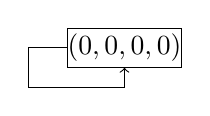
\begin{tikzpicture}[
		every node/.style = {
			draw, rectangle, 
			minimum width=0.75cm,
			minimum height=0.5cm,
			outer sep=0cm, inner sep=0cm,
			node distance=0cm
		}
		]
		\node (s0) {$(0, 0, 0, 0)$};
		\draw[->] (s0.west) -- ++(-0.5,0) -- ++(0,-0.5) -| (s0.south);
	\end{tikzpicture}
\end{document}